\section{Implementacja}
\label{implementation}
W celu przeprowadzenia prac badawczych na temat konsekwencji zaproponowanych mechanizmów koniecznym było zaimplementowanie podstawowego kompilatora. 
W tym rozdziale zostanie opisana implementacja kompilatora, która służyła do testów języka, oraz jej nietypowe aspekty, wynikające z projektu C-=-1.

\subsection{Fazy kompilacji}
\label{Compilation_phases}
Ze względu na nietypową konstrukcję C-=-1, proces kompilacji musi być dłuższy oraz ostrożniej zaprojektowany niż w typowym statycznie typowanym języku programowania.
Ponieważ użytkownik ma pisać kod, który będzie modyfikował wewnętrzne struktury danych kompilatora, musi on wiedzieć, kiedy które jej elementy są gotowe.
Kolejność operacji wykonywanych przez kompilator staje się przez to częścią języka.
Proces kompilacji dzieli się na następujące etapy:
\begin{enumerate}
  \item Budowa reprezentacji pośredniej atrybutów
  \item Zebranie definicji funkcji i typów
  \item\label{compilation_step:attribute_attachment} Przyłączenie atrybutów
  \item Budowa reprezentacji pośredniej funkcji i typów
  \item Wykonanie meta-funkcji atrybutów
  \item Zastąpienie wyrażeń zawierających statyczną refleksję ich wynikami
  \item Zapisanie reprezentacji pośredniej pakietu
  \item (opcjonalne) Konwersja do postaci pośredniej LLVM i kompilacja do kodu maszynowego
\end{enumerate}

Współczesne kompilatory są typowo skonstruowane z trzech części: front-end, middle-end i back-end \cite{intro_to_compiler_design}.
Zadaniem front-endu jest analiza składni, weryfikacja typów oraz budowa reprezentacji pośredniej kodu. Middle-end, operując niej, dokonuje optymalizacji niezależnych od maszyny docelowej.
Na koniec back-end optymalizuje kod pod kątem konkretnej architektury procesora i generuje kod maszynowy.

Ze względu na nietypowe wymagania C-=-1, zastosowano nowy podział odpowiedzialności.
W przeciwieństwie do typowych języków programowania implementowany kompilator nie może wygenerować reprezentacji pośredniej programu w jednym kroku.
Etap \ref{compilation_step:attribute_attachment} procesu kompilacji może wpływać na wybór przeciążenia funkcji.
Ten aspekt został opisany dokładniej w rozdziale \ref{Attributes_mechanism_cm1}

Kompilator C-=-1 dzieli się na następujące części:
\begin{enumerate}
  \item Frontend
  \item Interpreter
  \item Optimiser
  \item Serializator
  \item Backend Interface
  \item Backend
\end{enumerate}
Część z tych komponentów nazywa się tak samo, jak w klasycznej architekturze. Jest to zabieg celowy, ponieważ pełnią one te same funkcje. 
Dodatkowe komponenty kompilatora, które zostały wydzielone to: Interpreter, Serializator oraz Back end Interface. % todo: italic
Nazwa Optimiser została wybrana, ponieważ wyrażenie 'middle-end' rzadko występuje w literaturze, a wybrany termin lepiej opisuje ten komponent.

Ponieważ istotnym elementem języka C-=-1 jest możliwość wykonywania kodu w czasie kompilacji, jednym z wydzielonych komponentów jest Interpreter.
Operuje on na CIR omówionej w rozdziale \ref{reprezentacja_posrednia}. Interpreter stanowi najważniejszy komponent kompilatora, ponieważ większość transformacji odbywa się za jego pomocą. Szczegółowe działanie tego komponentu jest opisane w rozdziale \ref{interpreter}.

\lstinline{Optimiser} został dodany do struktury kompilatora, aby zapewnić możliwość dalszego rozwoju i dla kompletności projektu. Nie został jednak zaimplementowany.

\lstinline{Serializator} jest odpowiedzialny za zapisywanie i odczytywanie struktur danych kompilatora z postaci tekstowej.
Serializowaną w ten sposób pakiet można dystrybuować za pomocą serwisu takiego jak NPM \cite{npm} oraz używać w innych projektach.
Większość współczesnych języków programowania ma powiązany ze sobą system do zarządzania zależnościami, przechowujący listę publicznie dostępnych pakietów.
Ponieważ zawartością takiego modułu jest serializowane, niezależne od platformy CIR, nie istnieje problem binarnej kompatybilności.
Kompilacja programu używając pakietów C-=-1 jest zbliżona do kompilowania programu C++ używając zależności wyłącznie w formie kodu źródłowego.
Cały program jest kompilowany tym samym narzędziem, na tej samej maszynie i z tymi samymi flagami. Serializator został dokładnie opisany w rozdziale \ref{serializer}.

Kompilator C-=-1 używa LLVM jako back-endu. W związku z tym, koniecznym jest przetłumaczenie CIR na reprezentację pośrednią LLVM (w dalszej części pracy nazywanej LLVMIR). Dlatego do kompilatora dodano element \lstinline{Backend Interface}, który dokonuje tej konwersji. Obydwa te komponenty są opisane w rozdziałach \ref{Backend_Interface} oraz \ref{implementation:backend}.

Diagram \ref{compilation_process_diagram} przedstawia ogólny proces kompilacji.
Kod użytkownika jest dzielony na dwie części: atrybuty i funkcje oraz typy.
Ten podział wynika z konieczności analizy metakodu przed przetworzeniem normalnego kodu programu.


\begin{figure}[]
  \caption{diagram procesu kompilacji języka C-=-1}
  \label{compilation_process_diagram}
  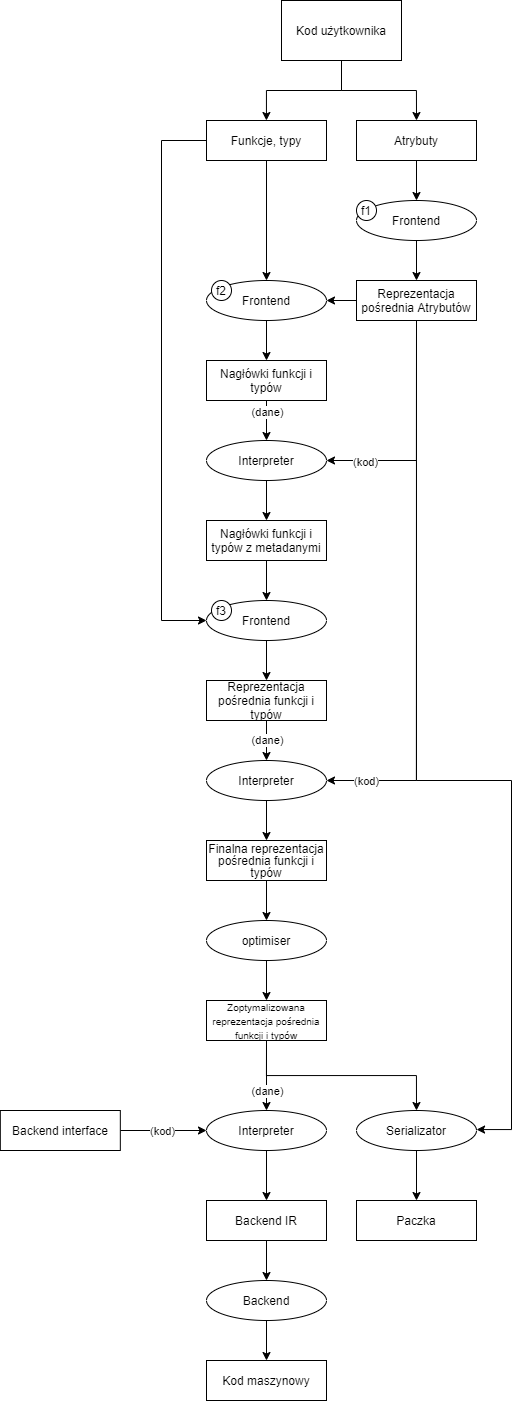
\includegraphics[width=\textwidth,height=\textheight,keepaspectratio]{img/compilation_process.png}
  \centering
\end{figure}

\subsection{Front-end}
Front-end kompilatora C-=-1 jest odpowiedzialny za analizę tekstu kodu źródłowego. Rysunek \ref{compilation_process_diagram} przedstawia diagram procesu kompilacji.
Front-end gra w nim kluczową rolę w początkowych fazach, przetwarzając zawartość plików źródłowych.
Sposób, w który źródła są odczytywane oraz analizowane jest opisany w rozdziale \ref{implementation:parser}.

Zrealizowanie tego procesu wymagało, aby ten komponent kompilatora potrafił funkcjonować w różnych trybach w zależności od obecnie wykonywanego kroku.
Ponadto, ponieważ w C-=-1, w przeciwieństwie do C++, kolejność deklaracji nie ma znaczenia, front-end musiał radzić sobie z zależnościami kołowymi.
Ogół działania front-endu jest opisany w rozdziale \ref{implementation:source_processing_phases}.

Frontend kompilatora jest również odpowiedzialny za tworzenie instancji atrybutów, kiedy przetwarza kod funkcji i typów.
Dlatego program użytkownika jest dzielony, przed analizą.
Przetworzenie typów i funkcji wymaga kompletnego modelu semantycznego atrybutów.

\subsubsection{Parser}
\label{implementation:parser}
Do analizy tekstu wejściowego, użyto generatora parserów Rose\cite{grabski2020}.
Jest to narzędzie bazujące na Antlr \cite{antlr}, które znacząco ułatwia manipulowanie drzewem składniowym (ang. Abstract Syntax Tree, AST).
Te dodatkowe możliwości są wykorzystywane przy przetwarzaniu szablonów (rozdział \ref{implementation:generics}).
Kompilator trzyma w pamięci tylko jedno drzewo rozkładu na raz, co oznacza, że każdy plik jest wczytywany wielokrotnie.
Ta decyzja ma ograniczyć ilość zużywanej w danym momencie pamięci operacyjnej.

\subsubsection{Fazy przetwarzania plików źródłowych}
\label{implementation:source_processing_phases}

Frontend kompilatora C-=-1 operuje w trzech fazach: \lstinline{create}, \lstinline{confirm} oraz \lstinline{finalize}.
Aby zapewnić, że kolejność deklaracji w programie nie ma znaczenia (w przeciwieństwie do C/C++), fazy są wykonywane dla wszystkich plików.
Najpierw wszystkie pliki przechodzą przez \lstinline{create}, potem przez \lstinline{confirm} a na koniec przez \lstinline{finalize}.

Faza \lstinline{create} zbiera nazwy bytów wewnątrz kodu aplikacji.
Tworzy wszystkie przestrzenie nazw, typy, funkcje oraz atrybuty.
W tym kroku kompilator nie analizuje zawartości tych obiektów.
Nie bierze pod uwagę pól i metod typów oraz parametrów i typów zwracanych funkcji.
Jeżeli w kodzie użytkownika istnieje na przykład funkcja mająca cztery przeciążenia, po fazie \lstinline{create} w modelu semantycznym będą istnieć cztery identyczne kopie tej deklaracji.

W fazie \lstinline{confirm} deklaracje są uzupełniane.
Do deklaracji funkcji dodawane są parametry i typ zwracany.
Typy są uzupełniane o pola oraz implementowane interfejsy.
Ponieważ na tym etapie kompilator zna wszystkie nazwy typów występujących w programie, kolejność deklaracji nie ma znaczenia, a deklaracje zapowiadające nie są konieczne.

W fazie \lstinline{finalize}
analizowane są ciała funkcji oraz metod.
Ten krok wykonywany jest na końcu, aby upewnić się, że kompilator jest w stanie rozwiązać przeciążenia wszystkich funkcji, do których odwołania mogą się pojawić.

\lstinline{Frontend} kompilatora C-=-1 działa w trzech trybach, w zależności od fazy kompilacji.
Na diagramie \ref{compilation_process_diagram} oznaczone zostały jako f1, f2 i f3.
W każdej z nich frontend zachowuje się inaczej.
\begin{itemize}
  \item W trybie f1 kompilator przechodzi przez wszystkie fazy i operuje wyłącznie na kodzie atrybutów.
  Funkcje oraz typy są ignorowane.
  \item W trybie f2 frontend przechodzi tylko przez fazy \lstinline{create} oraz \lstinline{confirm}, tylko na kodzie typów i funkcji.
  Przy okazji, korzystając z zebranych już informacji w trybie f1, tworzone są instancje atrybutów.
  \item W trybie f3 frontend wykonuje wyłącznie krok \lstinline{finalize} na funkcjach oraz metodach
\end{itemize}


\subsubsection{Zarządzanie zależnościami}

\subsubsection{Import symboli zewnętrznych}

\subsubsection{Reprezentacja pośrednia}
\label{implementation:intermidiate_representation}
Reprezentacja pośrednia jest istotnym elementem języka, na którym opiera się metaprogramowanie w C-=-1.
W związku, z czym każda jej część jest opisana w dokumentacji (załącznik 1).
Wewnątrz kompilatora, reprezentacja pośrednia jest przechowywana w ramach struktur danych interpretera (rozdział \ref{interpreter}), aby umożliwić jego modyfikację z interpretowanego programu.

Ponieważ użytkownik C-=-1 ma operować na CIR (C-=-1 Intermidiate Representation), jej struktura jest bliska językowi, który reprezentuje. 
Poza dodaniem specjalnych typów instrukcji struktura CIR jest niemal identyczna z C-=-1.
Takie podejście ma zarówno wady, jak i zalety. 
Z jednej strony sprawia ono, że błędy w kompilatorze są łatwiejsze do wykrycia, oraz front-end jest łatwiejszy do implementacji.
Przez podobieństwo reprezentacji pośredniej do kodu źródłowego, różnice względem poprawnego rezultatu są dużo bardziej oczywiste od bardziej abstrakcyjnych reprezentacji.
CIR jest jednak dużo trudniejsza do interpretowania.
W przeciwieństwie do języków takich jak CIL (Common Intermediate Language) \cite{ecma:cli}, CIR nie operuje abstrakcyjnej maszynie stosownej.
Szczegółowy opis działania interpretera znajduje się w rozdziale \ref{interpreter}.

Główne różnice w strukturze między C-=-1 a CIR polegają na bardziej dosłownym wyrażeniu programu. W reprezentacji pośredniej wszystkie odniesienia są w pełni kwalifikowane nazwą pakietu i przestrzenią nazw. Destruktory są wywoływane wprost, używając specjalnej instrukcji. Zamiast rozwiązywania przeciążeń funkcji, CIR odnosi się do konkretnego przeciążenia przez unikatowy identyfikator.

\subsubsection{Szablony}
\label{implementation:generics}



\subsection{Interpreter}
\label{interpreter}

Interpreter jest najważniejszym komponentem kompilatora C-=-1.
Diagram \ref{compilation_process_diagram} pokazuje, że w procesie kompilacji jest używany 3 razy (i1-i3).
Jest używany do konstrukcji atrybutów (i1), wykonywania operacji metaprogramistycznych (i2) oraz do generowania pliku wykonywalnego (i3).

Interpreter C-=-1 używa generycznych struktur danych opisanych w rozdziale \ref{implementation:interpreter:object_representation} zarówno jako danych, jak i reprezentacji wykonywanego programu.
Taka decyzja została podjęta, ponieważ częstym przypadkiem użycia tego komponentu jest modyfikacja programu, który niedługo będzie wykonywany.
Na przykład, jeśli kompilowany pakiet jest częścią większego projektu, kod modyfikowany w kroku i2, może, przy kompilacji następnego pakietu, zostać wykonany.
Wykonywanie kodu przez interpreter zostało dokładnie opisane w rozdziale \ref{implementation:interpreter:code_execution}.

To podejście ma jednak też swoje wady.
Ponieważ interpreter działa wyłącznie na generycznych strukturach danych, silne typowanie języka C++ nie jest w stanie wykryć pewnych błędów.
Ponadto, taka implementacja jest mniej efektywna niż użycie dedykowanych typów.

\subsubsection{Reprezentacja obiektów}
\label{implementation:interpreter:object_representation}

W kontekście działania interpretera C-=-1 przypomina bardziej dynamicznie typowany język skryptowy taki jak Python \cite{van1995python} niż statycznie typowany, kompilowany język jak C\# czy C++.
Interpreter działa na generycznych strukturach danych, typowych dla języka interpretowanego.
Rysunek \ref{implementation:data_structures:uml_diagram} przedstawia diagram UML klas używanych przez ten moduł.


\begin{figure}
  \caption{Diagram UML struktur danych interpretera C-=-1}
  \label{implementation:data_structures:uml_diagram}
  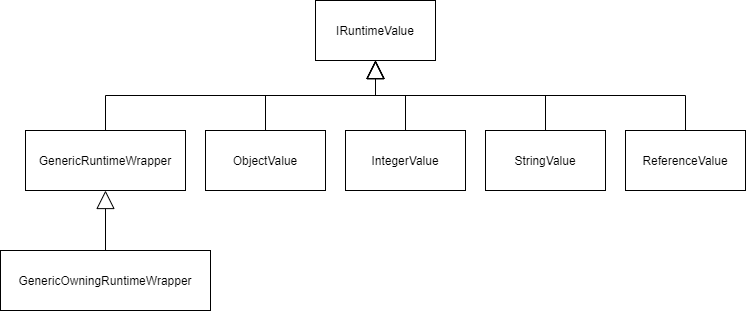
\includegraphics[width=\textwidth]{interpreter_data_structures_uml.png}
\end{figure}

\subsubsection{Wykonanie kodu}
\label{implementation:interpreter:code_execution}

\subsubsection{Funkcje specjalne}
\label{implementation:interpreter:special_functions}

\subsubsection{Referencje do obiektów C++}
\label{implementation:interpreter:cpp_object_references}

Umożliwienie C-=-1 modyfikacji modelu semantycznego programu, wymaga udostępnienie referencji do natywnych obiektów języka implementacji kompilatora. %todo: jesus fucking christ, wording
%todo: finish

\subsubsection{Biblioteka podstawowa}
\label{implementation:interpreter:basic_library}

Biblioteka podstawowa, w kontekście C-=-1, oznacza pakiet zawierający podstawowe funkcje oraz typy prymitywne.
W każdym języku programowania koniecznym jest specjalne traktowanie pewnego zbioru elementów programu takich jak prymitywne typy liczbowe czy funkcje arytmetyczne na nich.
W typowym kompilatorze wystarczy, że te obiekty zostaną uwzględnione przy generowaniu kodu.
Na przykład zamiast wywołania operatora plus dla dwóch liczb całkowitych, zostanie wstawiona instrukcja \lstinline{add}.

Ponieważ kompilator C-=-1 stanowi też jego pełne środowisko uruchomieniowe, musi zawierać wykonywalne definicje wszystkich operacji prymitywnych.
Ponadto, biblioteka podstawowa zawiera funkcję służące do komunikacji z kompilatorem, takie jak \lstinline{ignoreBody}, \lstinline{excludeAtRuntime}, \lstinline{excludeAtCompiletime}.
Służą one do modyfikowania metadanych funkcji przez atrybuty, co zostało dokładniej opisane w rozdziale \ref{Attributes_mechanism_cm1}.

Wszystkie funkcje z biblioteki podstawowej wymagają marshallingu, pomiędzy interpretowanym C-=-1 a środowiskiem uruchomieniowym w C++.
Ponieważ interpretowany C-=-1 działa na strukturach danych, opisanych w rozdziale \ref{implementation:interpreter:object_representation}, niekompatybilnych z C++, nie można użyć prostego rzutowania (poza przypadkiem z rozdziału \ref{implementation:interpreter:cpp_object_references}).

\begin{minipage}{\linewidth}
\begin{lstlisting}[
  numbers=left,
  firstnumber=0,
  caption={Przykład budowania funkcji z biblioteki podstawowej C-=-1},
  aboveskip=0pt,
  label={lst:marshalling_cm1}
  ]
void completeBuildingType(gsl::not_null<Type*> type) {
...
  createCustomFunction(
    type
    ->append<Function>("methods")
    ->setReturnType(TypeReference {
      getCollectionTypeFor(TypeReference{
        getFunctionDescriptor(), 0 
      }),
      0 
      }),
    type,
    [](
      map<string, unique_ptr<IRuntimeValue>>&& parameters,
      map<string, not_null<Type*>>genericParameters)
    {
      auto self = dereferenceAs<RuntimeTypeDescriptor>(
        parameters["self"].get())->value();
      auto methods = self.type->methods();
      return convertCollection(methods, TypeReference{
        getFunctionDescriptor(),
        0
      });
    }
  )->setAccessibility(Accessibility::Public);
...
}
\end{lstlisting}
\end{minipage}

Listing \ref{lst:marshalling_cm1} zawiera przykład budowania funkcji będącej częścią biblioteki podstawowej.
\lstinline{createCustomFunction} oznacza wybraną  funkcję jako zaimplementowaną natywnie w C++.
W liniach od trzeciej do dziesiątej, do deskryptora typu, dodawana jest metoda o nazwie \lstinline{methods}, zwracająca kolekcję deskryptorów funkcji.
W liniach od dwunastej do dwudziestej trzeciej tworzony jest obiekt funkcyjny lambda, który będzie służył jako ciało tej funkcji.
Ta procedura przyjmuje dwa argumenty: \lstinline{parameters} oraz \lstinline{genericParameters}.

Pierwszy z parametrów zawiera argumenty wywołania, indeksowane po nazwie parametru.
Na przykład dla wywołania \lstinline{f(1 + 1)} funkcji \lstinline{int f(int number)}, parametr \lstinline{parameters} pod kluczem \lstinline{number} zawierałby wartość 2.
W przykładzie z listingu \ref{lst:marshalling_cm1}, ponieważ zastępowane jest ciało metody, dostępna jest zmienna \lstinline{self}, będąca odpowiednikiem \lstinline{this} z C++.
Drugi parametr zawiera parametry generyczne, używane przy implementacji szablonów.

Linie od szesnastej do dwudziestej drugiej listingu \ref{lst:marshalling_cm1} zawierają kod wykonywany zamiast metody \lstinline{methods}.
Jego ogólna struktura jest dosyć typowa dla pod-programów w bibliotece podstawowej.
W liniach szesnastej i siedemnastej dochodzi do marshallingu ze struktur danych interpretera C-=-1 do natywnego obiektu C++.
W ten sposób pobierany jest obiekt deskryptora typu na, którym została wykonana ta metoda.
Zmienna \lstinline{self} ma więc typ \lstinline{TypeReference}, składający się z poziomu referencji oraz odniesienia do typu w modelu semantycznym.
Następnie, w linii osiemnastej, wywoływana jest metoda \lstinline{methods}, pobierająca wszystkie metody tego typu.
Na koniec, w linii dziewiętnastej dochodzi do marshallingu z natywnego \lstinline{vectora} C++ na kolekcję C-=-1.


\subsection{Serializator}
\label{serializer}

\subsection{Backend Interface}
\label{Backend_Interface}
Rolą interfejsu back-endu jest przetłumaczenie CIR na LLVMIR.
Na tym etapie kompilacji, cała reprezentacja pośrednia C-=-1 jest przechowywana w ramach struktur danych interpretera.
Stworzyło to okazję do napisania części kompilatora w języku docelowym.
To rozwiązanie zapewniło bezpieczeństwo typów w tej części kodu oraz ułatwiło rozwój C-=-1.
Tworzenie kompilatora w języku docelowym jest typowym w konstrukcji tego typu narzędzi.
Programy tak skonstruowane nazywają się 'Bootstrapping Compiler' \cite{puntambekar:compiler_design}. 

Implementacja tej części kompilatora w C-=-1 ułatwiła rozwój tego języka.
Jedną z głównych zalet narzędzia skonstruowanego w ten sposób jest istnienie dużego projektu w języku docelowym
Wymusza to szybszy rozwój języka oraz umożliwia znajdowanie błędów w kompilatorze.

\subsubsection{Funkcje eksponowane przez kompilator}

Używając mechanizmów, opisanych w rozdziałach \ref{implementation:interpreter:special_functions} oraz \ref{implementation:interpreter:cpp_object_references}, udostępniono interfejsowi backendu narzędzie do budowy LLVMIR zdefiniowane w LLVM.
W ramach biblioteki backendu istnieje cała gama funkcji oraz typów używanych do generowania reprezentacji pośredniej, co zostało opisane w rozdziale \ref{implementation:backend}.
W języku C-=-1 dostępny jest minimalny ich podzbiór, konieczny do implementacji podstawowego kompilatora.

\subsubsection{Implementacja interfejsu backendu}

Razem z plikiem wykonywalnym kompilatora, dystrybuowany jest kod źródłowy pakietu, zawierającej \emph{interfejs backendu}. 
Przed kompilacją kodu użytkownika, kompilator wczytuje ten moduł.
Zaletą tego rozwiązania jest możliwość wymiany tego komponentu, bez rekompilacji całego narzędzia.
Po załadowaniu tego pakiet kompilator szuka w niej funkcji oznaczonej atrybutem \lstinline{compilerEntryPoint}, która służy jako punkt wejścia dla interfejsu. 
Ma ona za zadanie wygenerowanie LLVMIR dla przekazanej jej listy pakietów (LLVMIR została opisana w rozdziale \ref{implementation:backend}).

Punkt wejścia \emph{interfejsu backendu} jako argumenty przyjmuje kolekcję pakietów do skompilowania oraz obiekt \lstinline{CompilationResult}.
Wynik kompilacji odpowiada kontekstowi LLVM, śledzi tworzone moduły oraz globalny stan LLVM.
Poza sygnaturą punktu wejścia, programista ma też obowiązek zapewnić specjalne traktowanie niektórych typów i funkcji z biblioteki podstawowej C-=-1, opisanej w rozdziale \ref{implementation:interpreter:basic_library}

\emph{Interfejs backendu} zaimplementowany w ramach tej pracy jest naiwny oraz niekompletny.
Nie wykorzystuje żadnych bardziej zaawansowanych mechanizmów LLVM oraz nie generuje metadanych dla debuggera.
Jego celem było zademonstrowanie możliwości języka C-=-1.

\subsection{Backend}
\label{implementation:backend}
Do generowania kodu maszynowego została wykorzystana biblioteka LLVM \cite{Lattner:MSThesis02}.
Ten pakiet jest obecnie używany jako backend całej rodziny języków C (C, C++, Objective-C) oraz języka Rust.
Aby wspierać tak szeroki zakres języków źródłowych, LLVM definiuje własną reprezentację pośrednią kodu: LLVMIR.

LLVMIR jest formą asemblera dla abstrakcyjnej maszyny stosowej \cite{llvmir}.
Program, zapisany w tej formie, jest dużo prostszy do automatycznej analizy i optymalizacji, oraz może zostać łatwiej skompilowany do kodu maszynowego dowolnego procesora.
Natomiast jego semantyczne podobieństwo do C, sprawia, że, stworzenie frontendu dla podobnego języka jest bardzo naturalne.

Maszyna abstrakcyjna LLVMIR operuje na typach, odpowiadającym strukturom z języka C bez nazwanych pól, oraz na funkcjach.
Funkcje mogą przyjmować nazwane parametry zarówno przez wartość, jak i wskazanie.
W LLVMIR nie istnieją wyrażenia złożone.
Wywołanie \lstinline{f(1 + 1)}, zapisane w C, należy wyrazić, najpierw jako deklaracja niemutowalnej zmiennej tymczasowej \lstinline{%0 = add i32 1, 1} a następnie jako wywołanie \lstinline{call void @f(i32 %0)}.

LLVMIR nie zawiera koncepcji mutowalnej zmiennej.
Wszystkie zmienne są wartościami stałymi i nie można ich modyfikować po przypisaniu.
Sposobem na zasymulowanie zachowania zmiennej z języka C, jest użycie instrukcji \lstinline{alloca}.
Alokuje ona miejsce na stosie, potrzebne dla danego typu i zwraca na nie wskazanie.
Programista może potem tę lokalizację w pamięci zmieniać oraz wczytywać jej wartość.

LLVM, poza kompilatorami LLVMIR do kodu maszynowego wielu różnych procesorów, zawiera też bibliotekę służącą do budowania LLVMIR.
Ten zestaw narzędzi jest bardzo przydatny, ponieważ dzięki niemu programista może operować na dobrze zdefiniowanej strukturze danych, zamiast na tekstowej reprezentacji.

\subsection{Biblioteka standardowa}

\subsection{Narzędzia dodatkowe}

\subsubsection{Tryb interaktywny}

\subsubsection{Debugger}

\subsubsection{Wtyczka do VS code}
\subsection{Wyzwania}
Generyki są zależne od kontekstu
Specjalne operatory nameof typeof etc
odchudzenie kompilatora przez trzymanie metadanych o funkcjach jako runtime value i funkcje do dostępu do tego jako klucz-wartość